% This is based on the LLNCS.DEM the demonstration file of
% the LaTeX macro package from Springer-Verlag
% for Lecture Notes in Computer Science,
% version 2.4 for LaTeX2e as of 16. April 2010
%
% See http://www.springer.com/computer/lncs/lncs+authors?SGWID=0-40209-0-0-0
% for the full guidelines.
%

\documentclass{llncs}
\usepackage{dsfont}
\newcommand{\argmin}{\operatornamewithlimits{argmin}}
\usepackage{graphicx}
\usepackage{booktabs}

\begin{document}


\title{To be defined}
%
\titlerunning{To be defined}  % abbreviated title (for running head)
%                                     also used for the TOC unless
%                                     \toctitle is used
%
\author{Author1 \and Author 2}
%
\authorrunning{Author1 et al.} % abbreviated author list (for running head)
%

%
\institute{LIMSI,\\
\email{email},\\ WWW home page:
\texttt{homepage}
}
\maketitle              % typeset the title of the contribution

\begin{abstract}
The abstract should summarize the contents of the paper
using at least 70 and at most 150 words. It will be set in 9-point
font size and be inset 1.0 cm from the right and left margins.
There will be two blank lines before and after the Abstract. \dots
\keywords{computational geometry, graph theory, Hamilton cycles}
\end{abstract}
%
\section{Dataset Presentation}

We obtained access to data gathered in home environment in three different housings. The energy consumption of the boiler was recorded without any control or advice given to the residents.
Two years of data are available for two homes and only one year for one boiler.
Measures were done on a ten minute basis. In our experiment, we use general information such as the ambient temperature in the housing, the outside temperature, the water temperature, the defrosting temperature and the state of the boiler (heating, waiting, etc).
\\Additionally, the temperature and the energy consumed between two records (10 minutes) is available for the EC1, EC2 and heating 1, heating 2. The dataset contains time information (day, hour, minute) and the house ID. 
\\Records were annotated with 2 possible labels,  namely : "1" and "2" which indicate whether hot water from the boiler was consumed durint the last ten minutes or not.
In total, we conduct our evaluation on 126 726 records and a total of 17 different features.

\section{Preprocessing \& Models} 
In this study, we compare supervised learning to semi-supervised learning to predict whether hot water was consumed or not. Our supervised model is a Deep-Neural Network (DNN). We apply automatic labeling and co-training as semi-supervised techniques.
To over-fitting and validate the performance of our approaches, we use 10-folds cross-validation on the data. In case of semi-supervised learning, only a subset of the labels of the training set is used.  
\\In addition to the label prediction, we performed data profiling to extract consumer behaviors in an unsupervised way. The goal is in future to help consumers to reduce their energy expenditure for example by integrating results in a coaching system. 
\subsection{Preprocessing}

Before learning or clustering the records we apply a preprocessing stage. 
\\We remove information related to time and the ID of the users. We found these information irrelevant and lead to a high over-fitting in case of training on them.
A few temperature and energy for the EC1 were missing, we fill the missing values with the average value of the field for the boiler.
We convert the "Graphset state" from categorical value to 5 boolean values, one for each possible state. 
For the supervised and semi-supervised approaches we convert the labels from (1,2) to two booleans values, to make training of a neural network easier. 



\subsection{Supervised Learning}

The first stage of the prediction of hot water consumption consists in data pre-processing followed by a learning classification stage. The purpose is to learn a mapping between the configuration of the features and the labels to be able in future to automatically guess the label.
\\In this study, the label prediction was done by applying a Deep-Neural Network (DNN). We compare the performance with a bagging classifier, a random forest classifier and a perceptron.
The results are also used as baseline for comparison with semi-supervised learning in Section 2.3. 
\\A Random Forest Classifier consists in a collection of weak learners known as decision trees. Each tree is trained on a sub samples of the dataset and a subset of features. The majority vote of the trees is taken as the decision of the random forest classifier. In our evaluation, we set the number of learners to 60.
\\A Bagging Classifier is a meta-estimator model which trains 20 k-nearest neighbors on subsets and subset of features of the dataset. The aggregation of the learners is similar to the random forest classifier. The main difference is in the subset construction made to reduce variance and improve learning. 
\\ Perceptron is the most simple neural network. Contrary to a DNN, its architecture is shallow, and doesn't contain hidden layers. The first layer of the neural network is directly connected to the output layer. The input layers has number of neurons equals to the number of features and the output layer to the number of classes. We set the regularization term to 0.0001.

Our main supervised approach is a deep neural network. 
Our Deep Neural Networks consists in a succession of fully connected layers. 
The input layer has a size equals to the number of features, 23 and is followed by several hidden layers. 
An hidden layer is a collection of units known as neurons connected to all the other neurons of the following layer.
The final layer consists in c neurons with c the number of possible classes. 
During propagation step, each layer receives as input the output of the previous layer and propagate the information to the next layer, from input to output layer. 
The output of the layer $l$ is computed as follow :
\begin{equation}
y^{(l)} = f^{(l)}(W^{(l)}x^{(l)})
\end{equation}
with $W^{(l)})$ the weights / parameters of the layer $l$, $x^{(l)}$ its input and $f^{(l)}$ an activation function.
During back propagation phase, information is propagate from the output layer (loss score) to the input layer and weights are updated in order to decrease loss.
\\An important issue in Deep-Neural Network named over-fitting occurs when the model is too closely fit to the training set which limits its generalization ability. As the neural network is deep compare to the number of features and the number of training epochs is large, we prevent it by using dropout and regularization.
\begin{figure}[tb]
\centering
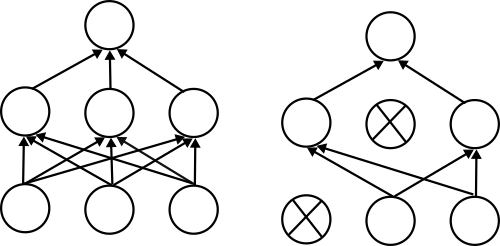
\includegraphics[width=0.7\linewidth]{images/dropout.png}
\caption{A neural without dropout (left) and with dropout (right)}
\label{fig:dropout-schema}
\end{figure}
Dropout turns-off neurons during training with a probability $p$ and at testing time, each neuron is scaled down by p. In case a neuron is turned-off, it is not taking in account during feed and forward pass.
The main effect is fighting against strongly correlated features and prevents co-adaptation between units. The idea behind is to avoid that the neurons learn to correct the neurons of the other neurons. Moreover, it forces each the neurons to be as general as possible and hence leads to a better generalization. 
\\ A new term called penalty term is added to the loss function in the regularization technique. Most used penalty terms are L1 and L2 terms, respectively defined as : 
\begin{equation}
L1\ term = \lambda + \sum\limits_{i=1}^k |w_{i}|
\end{equation}
L2 regularization term :
\begin{equation}
L2\ term = \lambda + \sum\limits_{i=1}^k w_{i}^{2}
\end{equation}
It prevents the coefficients to fit so perfectly to overfit and improve generalization.
\\Network was trained using the Adam algorithm, learning rate of $10^{-3}$, number of epochs 80 and minibatches of size 64. The architecture is composed by 4 hidden layers with a rectifier nonlinearity activation function and the size of the layers was set 20-30-30-30. The first layers is a fully connected layer with a size equal to the number of feature and a rectifier nonlinearity activation function. The output layer with a size 2, the number of classes to predict and a sigmoid function.
The parameters of the neural network were optimized using a binary cross-entropy loss function.
All our implementation are based on Keras library.
%ajouter details


\subsection{Semi-Supervised Learning}
We assume that data are difficult to annotate. In future, amount of data will highly increased requiring an important annotation work. To prevent this issue and make our model scalable to large datasets, we predict classes with a two different semi-supervised approaches, label-propagation and self-training.
We train the models on a small subset of labeled data enhanced by a large amount of unlabeled data. In our experiment, we consider that 20\% of the training examples are labeled and 80\% of data are not annotated. 

\subsubsection{Label Propagation}

\begin{figure}[tb]
\centering
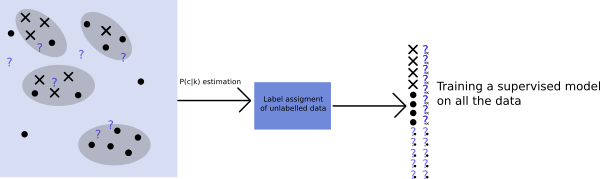
\includegraphics[width=1.0\linewidth]{images/labelPropagation.png}
\caption{Label Propagation approach}
\label{fig:label-propagation}
\end{figure}


This approach increases the number of annotated data by estimating the most probable class of the non-annotated data. 
The algorithm is divided in three stages, compute clusters, estimate the probability of a class within each cluster and train a supervised model. 
In order to assign labels, we generate $k$ clusters from the labeled data. We believe that data with a same label will be grouped in the same clusters.


For each cluster, we compute the probability of a class $c$ given a cluster $K$ as:

\begin{equation}
\label{proba-cluster}
P(c|K) = \sum\limits_{x\in K} 1I_{label(x)=c}*P(c) /|K|
\end{equation}

We estimate the probability of a class $c$, $P(c)$ as the number of data with the label $c$ within the training set. As can be seen in Equation \ref{proba-cluster}, if a class $c'$ is not represented, the probability $P(c'|k)$ is equal to zero. 
To annotate data, we firstly assign a cluster to each unlabeled data. This case depends of the algorithms used for the clustering. In case of K-means, the closest cluster is selected.
For each point to labelize and its associated cluster $k$, we sample a label over the classes $C$ by following a distribution given by the probabilities $P(c|k)$.

The last stage of the training process consists in training a Deep Neural Network to predict the class. The DNN architecture is the same as described in the fully supervised approach. We keep the same parameters to make the comparison fare.
As we have labeled data, the number of data is same as if we were in a supervised context. 
\\In our experiment, we use expectation-maximization for gaussian mixtures algorithm to generate the clusters. This technique gives the most coherent clusters.  

\subsubsection{Co-Training}
Co training is an algorithm that gradually increases the number of annotated data by automatically assign missing labels.
A supervised classifier is trained on the labeled data. This model is used to predict label of a small subset of unlabeled data. The new labeled data with a high confidence score are added to the training set of the supervised model.
This procedure is repeated and the supervised model retrained until convergence. 

\subsection{Unsupervised Learning}

In this section, we perform automatic profiling.
Additionally to the prediction task, we want to extract consumption behaviors and group them. In future, the profiling could be used by a coaching model for example to help to reduce energy consumption of a housing or to to characterize a boiler based on several records and the clusters to which it belongs.  
We compare two unsupervised approaches, K-means clustering and mixture of gaussians with expectation-maximization without accessing and extract consumption characteristics from the obtained clusters. 

\subsubsection{K-Means}

K-means aims to group the data in several clusters $C$ based on similarity of the features. Iteratively, the clusters are updated until convergence or a number of epochs is reached. A cluster $c_{i}$ is represented by its centroid.
First, the algorithms randomly selects $k$ centroids. At each time-step, the algorithm assigns to each data $x$ a cluster based on its distance to the clusters.
\begin{equation}
\label{min-distance}
	argmin_{c_{i}\in C} dist(c_{i},x)
\end{equation}
with $dist(c_{i},x)$ distance between the cluster and the point. 
After the assignment step, the clusters / centroids are updated by taking mean of all points assigned to the clusters :
\begin{equation}
c_{i} = \frac{1}{|S_{i}|}\sum\limits_{x_{i} \in C_{i}} x_{i}
\end{equation}
We found that a number of iterations equal to 1000 and K=3 gives the most coherent clusters. To initialize the centroids, we randomly select data from our dataset without taking into account the label. We use the cosine similarity as distance function in the Equation \ref{min-distance}.


\subsubsection{Expectation-Maximization for Gaussian Mixtures}

Expectation–Maximization (EM) for Gaussian Mixtures is a clustering method with soft-assignment, a probability distribution of assignment over the clusters. 
Each cluster is represented by a gaussian distribution with parameters $\theta_{k}=$ \{$\mu_{k},\sum_{k}$\}.
Two phases are iteratively repeated until convergence : an expectation phase and a maximization phase to estimate the paramters of the mixtures of gaussian. 
During the E-phase, the membership weight of a point $x_{i}$ to a cluster $k$ given parameters $\Theta$ is defined as
\begin{equation}
w_{ik} = p(z_{ik} = 1|x_{i},\Theta)= \frac{p_{k}(x_{i}|z_{k},\theta_{k})\cdot \alpha_{k}}{\sum\limits_{m=1}^K p_{m}(x_{i}|z_{m},\theta_{m})\cdot \alpha_{m}}, 1\leq k\leq K, 1\leq i\leq N.
\end{equation}
This estimation is done for all records $x_{i}, 1\leq i\leq N$ and all mixture components $1\leq k\leq K$. Since the weights are probabilities of assignment, the sum of the weights of a point is equal to 1.
The parameters of the mixtures of gaussians are then updated according to the new weights. The mean of the gaussians is calculated as an average:
\begin{equation}
\mu_{k}^{new} = (\frac{1}{N_{k}}) \sum\limits_{i=1}^N w_{ik}\cdot x_{i}, 1\leq k \leq K
\end{equation}
And the covariance matrix are updated similarly :
\begin{equation}
\sum_{k}^{new} = \frac{1}{N_{k}} \sum\limits_{i=1}^N
 w_{ik} \cdot (x_{i} - \mu_{k}^{new})(x_{i}-\mu_{k}^{new})^{t}, 1\leq k \leq K \end{equation}

In order to detect the convergence, we compute log-likelihood and set threshold ratio to stop algorithm to $10^{-3}$. To improve convergence the weights are not randomly initialized but using K-means.  

\section{Results \& Discussions}
%In the following, we report and compare the results of the supervised algorithms against the semi-supervised approaches. We use 

\subsection{Supervised Learning}

In the following, we report the results of the supervised algorithms. To evaluate our approach we use the accuracy as error metric. We used $k$-fold validation with $k=10$ to have a robust evaluation. 
We optimized the DNN parameters, by sampling hyper-parameters from categorical distributions:

\begin{itemize}
\item Number of hidden layers from $[1,5]$
\item Size of hidden layers from $[10,100]$
\item Dropout probability $\{0,10,20,30,40,50,60,70\}$ 
\end{itemize}

The best hyper parameters is a neural network with 4 hidden layers of size 20-30-30-30 and a dropout probability of $0.5$. 
\\Additionally, we report the accuracy of the DNN with and without dropout and regularization to exhibit impact on over-fitting. 
\begin{table}
\centering
  \caption{Impact of the regularization on the testing performance}
  \label{tab:performance-regu}
  \begin{tabular}{ccl}
    \toprule
    Settings&Training accuracy&Testing accuracy\\
    \midrule
    DDN & 82.413&77.357\\
    DNN + dropout & 90.088&91.228\\
    DNN + l1 regularization & 85.003&84.905\\
    DNN + l2 regularization & 86.200&86.145\\
    DNN + l2 regularization + dropout & 96.241&96.052\\
  \bottomrule
\end{tabular}
\end{table}

\begin{figure}[tb]
\centering
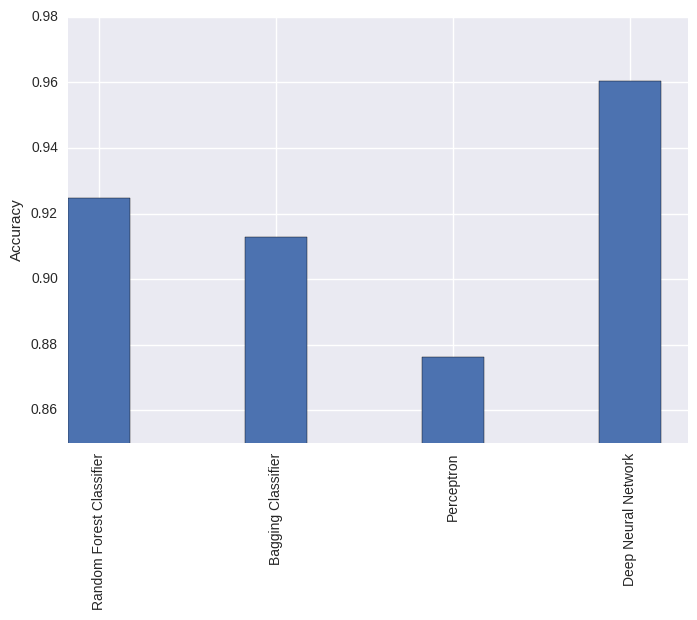
\includegraphics[width=0.8\linewidth]{images/res-algos.png}
\caption{Accuracy of the supervised algorithms}
\label{fig:supervised-scores}
\end{figure}

The Figure \ref{fig:supervised-scores} reports the accuracy of the supervised algorithms. As can be seen, our DNN performs better than all the other models in term of accuracy. We can also observe that using a deep neural network architecture achieves a significantly higher accuracy than the perceptron, a neural network with a shallow architecture.


\subsection{Semi-supervised Learning}

\subsubsection{Label Propagation}

Figure XXX shows performance of this approach. Our supervised model uses the same deep neural network architecture as the one described in the supervised learning technique. 
We varied the number of clusters in the k-means model and measure accuracy. 
We can observe that increasing....

%
%DIFFERENT NOMBRE DE CLUSTERS
%FAIRE VARIER POURCENTAGE DONNEES NON LABELISEE
%We report in Figure XXX the accuracy when varying the percentage of labelled data avaible for training with a number of clusters fix to XXX.




\subsection{Profiling}

Evaluating performance without using labels is difficult. Moreover, manually evaluating the coherence of the clusters would be too subjective. In our experiments, we used the Calinski Harabaz criterion which evaluates the ratio between the dispersion within the clusters and the dispersion of the clusters. 

\begin{equation}
CH(k)= \frac{B_{c}(k)}{(k-1)}/\frac{W_{c}(k)}{(n-1)}
\end{equation}k
with n the number of centroids and k the number of different labels, $B_{c}$ and $W_{c}$ the dispersion between and within clusters respectively. 
\begin{equation}
B_{c} = \sum\limits_{k=1}^K |C_{k}| ||\bar{C_{k}} - \bar{x}||^{2}
\end{equation}
\begin{equation}
W_{c} = \sum\limits_{k=1}^K\sum\limits_{i=1}^N w_{k,i} ||x_{i} - \bar{C_{k}}||^{2}
\end{equation}

\subsubsection{K-means}

\begin{figure}[tb]
\centering
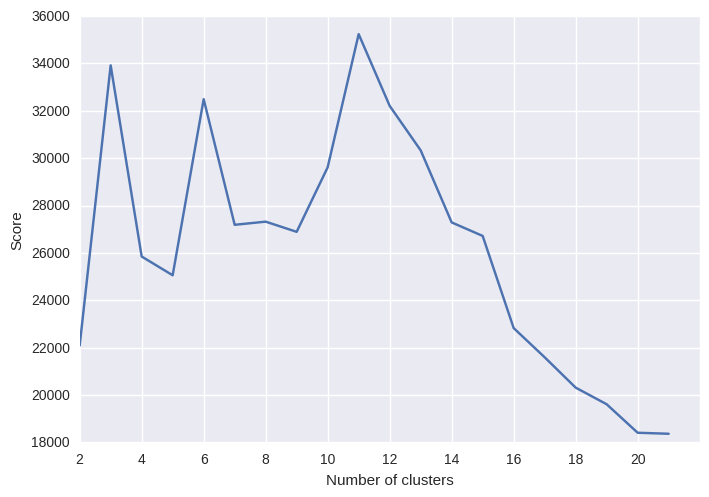
\includegraphics[width=0.8\linewidth]{images/clusters_K-means.png}
\caption{Calinski Harabaz for different number of clusters obtained by the K-means algorithm and the cosinne similarity as distance function}
\label{fig:kmeans-scores}
\end{figure}


As can be seen in Figure \ref{clusters_K-means}, the optimal number of clusters is $K=3$. We also evaluate the clusters by manually checking the characteristics. We observed that the algorithm successfully create clusters with characteristics. For example, the records in clusters 1 have a low outside temperature and a low defrosting temperature whereas records in cluster 2 have a moderated outside temperature and a high energy consumption on the ECS2. 

\subsubsection{Expectation-Maximization for Gaussian Mixtures}

\begin{figure}[tb]
\centering
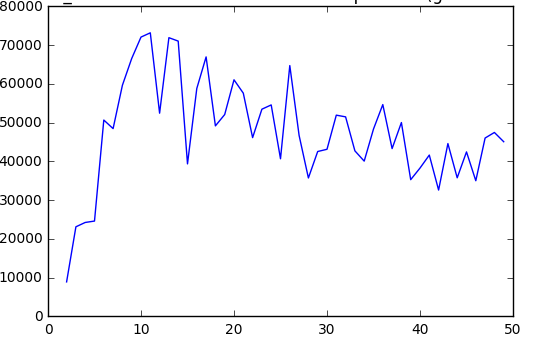
\includegraphics[width=0.8\linewidth]{images/clusters_EM.png}
\caption{Calinski Harabaz for different number of clusters obtained by the EM with mixture of gaussians algorithm}
\label{fig:em-scores}
\end{figure}

Figure \ref{fig:em-scores} shows that the Calinski Harabaz score reaches a maximum for a number of mixtures equals to 11. A higher number of mixtures leads to a lower score which mean a larger dispersion within the clusters and a smaller dispersion between the clusters. We can observe that the score has a high fluctuation which make the choice of the number of mixtures difficult.

Similarly to the k-means, we checked the characteristics. Since the number of clusters is higher, we can extract more accurate characteristics for each cluster. For example, the cluster 4 and 8 are the only one with a high energy consumption of the heating 1 or the clusters 1 and 8 are clusters with an average outside temperature below 0°C.  

Since comparing the Calinski Harabaz scores of the K-means and expectation-maximization for gaussian mixtures algorithms is not relevant, we use manual checking. We believe that the clusters obtained by the EM with gaussian mixtures are more coherents but this evaluation is not totally objective and could be improved.


%
% ---- Bibliography ----
%
\begin{thebibliography}{5}
%


\end{thebibliography}

\end{document}
